\documentclass{article}
\usepackage[utf8]{inputenc}
\usepackage[english]{babel}
\usepackage[]{amsthm} 
\usepackage[]{amssymb} 
\usepackage{amsmath}
\usepackage{hyperref}
\usepackage{multirow}
\usepackage{tabularx}
\usepackage{graphicx}
\graphicspath{ {./solution_images/} }
\usepackage{float}
\usepackage{karnaugh-map}
\usepackage{listings}
\usepackage{tikz}
\usetikzlibrary{automata, positioning, arrows}
\tikzset{
    ->, % makes the edges directed
    node distance=3cm, % specifies the minimum distance between two nodes. Change if necessary.
    every state/.style={thick, fill=gray!10}, % sets the properties for each ’state’ node
    }
\usepackage{subcaption}
\usepackage[table]{xcolor}
\usepackage[dvipsnames]{xcolor}
\usepackage[thinc]{esdiff}


\title{Digital System Design and Lab: HW4}
\author{Lo Chun, Chou \\ R13922136}
\date\today

\begin{document}
\setlength{\parindent}{0pt}
\maketitle 

\section*{1}
\subsection*{(1)}

\begin{table}[H]
    \centering
    \resizebox{0.4\textwidth}{!}{
        \begin{tabular}{|c|c|c||c|c|c|}
            \hline
            \multicolumn{3}{|c||}{Present State} & \multicolumn{3}{c|}{Next State} \\
            \hline
            $C$ & $B$ & $A$ & $C^+$ & $B^+$ & $A^+$ \\
            \hline
            0 & 0 & 1 & 0 & 1 & 1 \\
            0 & 1 & 1 & 0 & 1 & 0 \\
            0 & 1 & 0 & 1 & 1 & 0 \\
            1 & 1 & 0 & 1 & 1 & 1 \\
            1 & 1 & 1 & 1 & 0 & 1 \\
            1 & 0 & 1 & 1 & 0 & 0 \\
            1 & 0 & 0 & 0 & 0 & 1 \\
            \hline
        \end{tabular}
        }
    \end{table}

\begin{figure}[H]
    \centering
    \begin{subfigure}{0.3\textwidth}
        \centering
        \begin{karnaugh-map}[2][4][1][$C$][$A$][$B$]
            \terms{0}{X}
            \minterms{3, 4, 5, 7}
            \maxterms{1, 2, 6}
        \end{karnaugh-map} 
        \caption{$C^+$}
    \end{subfigure}
    \begin{subfigure}{0.3\textwidth}
        \centering
        \begin{karnaugh-map}[2][4][1][$C$][$A$][$B$]
            \terms{0}{X}
            \minterms{2, 4, 5, 6}
            \maxterms{1, 3, 7}
        \end{karnaugh-map} 
        \caption{$B^+$}
    \end{subfigure}
    \begin{subfigure}{0.3\textwidth}
        \centering
        \begin{karnaugh-map}[2][4][1][$C$][$A$][$B$]
            \terms{0}{X}
            \minterms{1, 2, 5, 7}
            \maxterms{3, 4, 6}
        \end{karnaugh-map} 
        \caption{$A^+$}
    \end{subfigure}
    \caption{K-maps}
\end{figure}
\newpage

\subsection*{(2)}

The K-maps for D flip-flop are the same as the K-maps for $C^+$, $B^+$, and $A^+$ in (1), 
since we assign the values of $D_C$, $D_B$, and $D_A$ to be $C^+$, $B^+$, and $A^+$ respectively.
\bigskip

Thus, the following $D_C$ is the same as $C^+$:

\begin{figure}[H]
    \centering
    \begin{karnaugh-map}[2][4][1][$C$][$A$][$B$]
        \terms{0}{X}
        \minterms{3, 4, 5, 7}
        \maxterms{1, 2, 6}
        \implicant{3}{7}
        \implicant{4}{5}
    \end{karnaugh-map} 
    \caption{D flip-flop ($D_C$)}
\end{figure}

The minimum SOP expression for $D_C$ is:

\begin{align*}
    D_C = AC + A'B 
\end{align*}
\newpage

\subsection*{(3)}

Since $C$ is toggled for $CBA = \{010, 100\}$, we can derive the following K-map for $T_C$:

\begin{figure}[H]
    \centering
    \begin{karnaugh-map}[2][4][1][$C$][$A$][$B$]
        \terms{0}{X}
        \minterms{1, 4}
        \maxterms{2, 3, 5, 6, 7}
        \implicant{0}{1}
        \implicantedge{0}{0}{4}{4}
    \end{karnaugh-map} 
    \caption{T flip-flop ($T_C$)}
\end{figure}

The minimum SOP expression for $T_C$ is:

\begin{align*}
    T_C = A'B' + A'C'
\end{align*}
\newpage

\subsection*{(4)}

From the truth table is subproblem $(1)$, we have:

\begin{align*}
    \{B, B^+\} = 
    \begin{cases}
        \{0, 0\} & \text{for } CBA = \textcolor{blue}{\{101, 100\}} \rightarrow \{S, R\} = \textcolor{Green}{\{0, X\}} \\
        \{0, 1\} & \text{for } CBA = \textcolor{blue}{\{001\}} \rightarrow \{S, R\} = \textcolor{Green}{\{1, 0\}} \\
        \{1, 0\} & \text{for } CBA = \textcolor{blue}{\{111\}} \rightarrow \{S, R\} = \textcolor{Green}{\{0, 1\}} \\
        \{1, 1\} & \text{for } CBA = \textcolor{blue}{\{011, 010, 110\}} \rightarrow \{S, R\} = \textcolor{Green}{\{X, 0\}}
    \end{cases}
\end{align*}

\begin{figure}[H]
    \centering
    \begin{subfigure}{0.4\textwidth}
        \centering
        \begin{karnaugh-map}[2][4][1][$C$][$A$][$B$]
            \terms{0, 4, 5, 6}{X}
            \minterms{2}
            \maxterms{1, 3, 7}
            \implicant{0}{4}
        \end{karnaugh-map} 
        \caption{$S_B$}
    \end{subfigure}
    \begin{subfigure}{0.4\textwidth}
        \centering
        \begin{karnaugh-map}[2][4][1][$C$][$A$][$B$]
            \terms{0, 1, 3}{X}
            \minterms{7}
            \maxterms{2, 4, 5, 6}
            \implicant{3}{7}
        \end{karnaugh-map} 
        \caption{$R_B$}
    \end{subfigure}
\end{figure}

The minimum SOP expression for $S_B, R_B$ are:

\begin{align*}
    &S_B = C' \\
    &R_B = AC
\end{align*}
\newpage

\subsection*{(5)}

From the truth table is subproblem $(1)$, we have:

\begin{align*}
    \{A, A^+\} = 
    \begin{cases}
        \{0, 0\} & \text{for } CBA = \textcolor{blue}{\{010\}} \rightarrow \{J, K\} = \textcolor{Green}{\{0, X\}} \\
        \{0, 1\} & \text{for } CBA = \textcolor{blue}{\{110, 100\}} \rightarrow \{J, K\} = \textcolor{Green}{\{1, X\}} \\
        \{1, 0\} & \text{for } CBA = \textcolor{blue}{\{011, 101\}} \rightarrow \{J, K\} =  \textcolor{Green}{\{X, 1\}} \\
        \{1, 1\} & \text{for } CBA = \textcolor{blue}{\{001, 111\}} \rightarrow \{J, K\} = \textcolor{Green}{\{X, 0\}}
    \end{cases}
\end{align*}

\begin{figure}[H]
    \centering
    \begin{subfigure}{0.4\textwidth}
        \centering
        \begin{karnaugh-map}[2][4][1][$C$][$A$][$B$]
            \terms{0, 2, 3, 6, 7}{X}
            \minterms{1, 5}
            \maxterms{4}
            \implicant{1}{5}
        \end{karnaugh-map} 
        \caption{$J_A$}
    \end{subfigure}
    \begin{subfigure}{0.4\textwidth}
        \centering
        \begin{karnaugh-map}[2][4][1][$C$][$A$][$B$]
            \terms{0, 1, 4, 5}{X}
            \minterms{3, 6}
            \maxterms{2, 7}
            \implicant{1}{3}
            \implicant{6}{4}
        \end{karnaugh-map} 
        \caption{$K_A$}
    \end{subfigure}
\end{figure}

The minimum SOP expression for $J_A, K_A$ are:

\begin{align*}
    &J_A = C \\
    &K_A = BC' + B'C
\end{align*}
\newpage

\section*{2}

\subsection*{(1)}

Following the steps to construct the state table at lecture slides 13, p. 15, 
we first determine the flip-flop and output equations:

\begin{align*}
    &\textcolor{orange}{J_1} = \textcolor{orange}{X}, \\ 
    &\textcolor{Green}{K_1} = X \barwedge Q_2' = (XQ_2')' = \textcolor{Green}{X' + Q_2}, \\
    &\textcolor{orange}{J_2} = \textcolor{orange}{X}, \\
    &\textcolor{Green}{K_2} = Q_1 \barwedge X = (Q_1X)' = \textcolor{Green}{Q_1' + X'}, \\
    &\textcolor{blue}{Z} = Q_2' \oplus X = \textcolor{blue}{Q_2'X' + Q_2X}
\end{align*}

Then, using the next state equation for JK flip-flop, which is:

\begin{align*}
    Q^+ = JQ' + K'Q
\end{align*}

we have:

\begin{align*}
    &Q_1^+ = J_1Q_1' + K_1'Q_1 = XQ_1' + (X' + Q_2)'Q_1 = \underline{XQ_1' + XQ_1Q_2'} \\
    &Q_2^+ = J_2Q_2' + K_2'Q_2 = XQ_2' + (Q_1' + X')'Q_2 = \underline{XQ_2' + XQ_1Q_2} \\
    &Z = \underline{Q_2'X' + Q_2X}
\end{align*}

We then plot the next state map for each flip-flop:

\begin{figure}[H]
    \centering
    \begin{subfigure}{0.33\textwidth}
        \centering
        \begin{karnaugh-map}[2][4][1][$X$][$Q_2$][$Q_1$]
            \minterms{1, 3, 5}
            \maxterms{0, 2, 4, 6, 7}
            \implicant{1}{3}
            \implicantedge{1}{1}{5}{5}
        \end{karnaugh-map} 
        \caption{$Q_1^+$}
    \end{subfigure}
    \begin{subfigure}{0.33\textwidth}
        \centering
        \begin{karnaugh-map}[2][4][1][$X$][$Q_2$][$Q_1$]
            \minterms{1, 5, 7}
            \maxterms{0, 2, 3, 4, 6}
            \implicantedge{1}{1}{5}{5}
            \implicant{7}{5}
        \end{karnaugh-map}
        \caption{$Q_2^+$}
    \end{subfigure}
    \begin{subfigure}{0.3\textwidth}
        \centering
        \begin{karnaugh-map}[2][4][1][$X$][$Q_2$][$Q_1$]
            \minterms{0, 3, 4, 7}
            \maxterms{1, 2, 5, 6}
            \implicantedge{0}{0}{4}{4}
            \implicant{3}{7}
        \end{karnaugh-map}
        \caption{$Z$}
    \end{subfigure}
\end{figure}

We can then use the K-maps to form the state table:

\begin{table}[H]
    \centering
    \begin{tabular}{|c||c|c||c|c|}
        \hline
        \multirow{2}{*}{$Q_1Q_2$} & \multicolumn{2}{c||}{$Q_1^+Q_2^+$} & \multicolumn{2}{c|}{$Z$} \\
        \cline{2-5}
        & $X = 0$ & $X = 1$ & $X = 0$ & $X = 1$ \\
        \hline
        $00$ & 00 & 11 & 1 & 0 \\
        \hline
        $01$ & 00 & 10 & 0 & 1 \\
        \hline
        $11$ & 00 & 01 & 0 & 1 \\
        \hline
        $10$ & 00 & 11 & 1 & 0 \\
        \hline
    \end{tabular}
\end{table}

\subsection*{(2)}

We first replace part of the resulting state table in subproblem $(1)$ with the following symbols:

\begin{align*}
    S_0 = 00, \quad S_1 = 01, \quad S_2 = 11, \quad S_3 = 10
\end{align*}

Then we'll have:

\begin{table}[H]
    \centering
    \begin{tabular}{|c||c|c||c|c|}
        \hline
        \multirow{2}{*}{$Q_1Q_2$} & \multicolumn{2}{c||}{$Q_1^+Q_2^+$} & \multicolumn{2}{c|}{$Z$} \\
        \cline{2-5}
        & $X = 0$ & $X = 1$ & $X = 0$ & $X = 1$ \\
        \hline
        $S_0$ & $S_0$ & $S_2$ & 1 & 0 \\
        \hline
        $S_1$ & $S_0$ & $S_3$ & 0 & 1 \\
        \hline
        $S_2$ & $S_0$ & $S_1$ & 0 & 1 \\
        \hline
        $S_3$ & $S_0$ & $S_2$ & 1 & 0 \\
        \hline
    \end{tabular}
\end{table}

Using this table, we can construct the state diagram:

\begin{figure}[H]
    \centering
    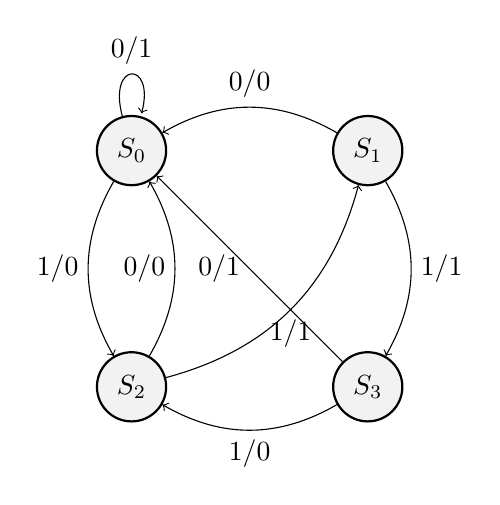
\begin{tikzpicture}
        \node[state] (q00) {$S_0$};
        \node[state] (q01) [right of=q00] {$S_1$};
        \node[state] (q11) [below of=q00] {$S_2$};
        \node[state] (q10) [right of=q11] {$S_3$};

        \draw (q00) edge[loop above] node{$0 / 1$} (q00);
        \draw (q00) edge[bend right, left] node{$1 / 0$} (q11);
        \draw (q01) edge[bend right, above] node{$0 / 0$} (q00);
        \draw (q01) edge[bend left, right] node{$1 / 1$} (q10);
        \draw (q11) edge[bend right, left] node{$0 / 0$} (q00);
        \draw (q11) edge[bend right, below] node{$1 / 1$} (q01);
        \draw (q10) edge[left] node{$0 / 1$} (q00);
        \draw (q10) edge[bend left, below] node{$1 / 0$} (q11);
    \end{tikzpicture}
\end{figure}
\newpage

\section*{3}

\subsection*{(1)}

From the following image, we can check that for all possible situations $0000$ to $1111$, 
what the next state should be after the input $X = \{0, 1\}$ is applied.

\begin{figure}[H]
    \centering
    \includegraphics[width=0.7\textwidth]{3_1.jpeg}
\end{figure}

Let $S_0$ be the initial state, which assumes all previous inputs were $0$ as given in the problem.
We then add two states $S_1$ and $S_2$ to represent the cases when the current input along with the previous $3$ inputs is valid and invalid respectively.

\bigskip
This also means that the green states in the above image would go to $S_1$ and the red states would go to $S_2$.
\bigskip

Thus, we can form the state table as follows:

\begin{table}[H]
    \centering
    \begin{tabular}{|c||c|c||c|c|}
        \hline
        \multirow{2}{*}{Current State} & \multicolumn{2}{c||}{Input} & \multicolumn{2}{c|}{$Z$} \\
        \cline{2-5}
        & $X = 0$ & $X = 1$ & $X = 0$ & $X = 1$ \\
        \hline
        $S_0$ & $S_0$ & $S_1$ & 0 & 0 \\
        \hline
        $S_1$ & $S_1$ & $S_1, S_2$ & 0 & 0 \\
        \hline
        $S_2$ & $S_1, S_2$ & $S_1, S_2$ & 1 & 1 \\
        \hline
    \end{tabular}
\end{table}
\newpage

\subsection*{(2)}

We shall use the following four states, with each of them containing the previous $4$ inputs as follows:

\begin{align*}
    &S_0 = \{0000, 0001, 0010, 0011\} \\
    &S_1 = \{0100, 0101, 0110, 0111\} \\
    &S_2 = \{1000, 1001\} \\
    &S_3 = \{1010, 1011, 1100, 1101, 1110, 1111\}
\end{align*}

For $S_0$, this state contains all the cases when no matter we receive any input ($X = 0$ or $1$), it would still be valid. 
\bigskip

For $S_1$, this state contains the cases when it receives $0$ as input, it would go to $S_0$, and would be invalid (go to $S_3$) if it receives $1$.
\bigskip

For $S_2$, this state contains the cases when it receives $0$ as input, it would go to $S_1$, and would be invalid (go to $S_3$) if it receives $1$. (The distinction between $S_1, S_2$ is that it is possible for $S_1$ to enter the next state $S_0$, which would be valid no matter what next input is.)
\bigskip

For $S_3$, this state contains all the invalid cases. 
\bigskip

We can then form the state table as follows:

\begin{table}[H]
    \centering
    \begin{tabular}{|c||c|c||c|c|}
        \hline
        \multirow{2}{*}{Current State} & \multicolumn{2}{c||}{Input} & \multicolumn{2}{c|}{$Z$} \\
        \cline{2-5}
        & $X = 0$ & $X = 1$ & $X = 0$ & $X = 1$ \\
        \hline
        $S_0$ & $S_0$ & $S_0$ & 0 & 0 \\
        \hline
        $S_1$ & $S_0$ & $S_3$ & 0 & 1 \\
        \hline
        $S_2$ & $S_1$ & $S_3$ & 0 & 1 \\
        \hline
        $S_3$ & $S_1$ & $S_3$ & 0 & 1 \\
        \hline
    \end{tabular}
\end{table}


\newpage

\section*{4}

\subsection*{(1)}

The following screenshot is the module \lstinline{mult_fast}

\begin{figure}[H]
    \centering
    \includegraphics[width=0.7\textwidth]{4_1.png}
\end{figure}

And also not required, the following figure shows how the indices are decided:

\begin{figure}[H]
    \centering
    \includegraphics[width=0.7\textwidth]{4_1_design_process.jpeg}
\end{figure}

\subsection*{(2)}

\begin{figure}[H]
    \centering
    \includegraphics[width=\textwidth]{4_2.png}
\end{figure}

\subsection*{(3)}

We can find the latency by the above waveform, for example, 
if we look at the input at the input at $1750$, we have inputs $A = 1010$ and $B = 1110$, 
which corresponds to $10$ and $14$ respectively.
\bigskip

Thus, the output $P$ at $1750$ is $10 \times 14 = 140$, which can be represented as $10001100$ in binary, 
and this correct product appears at $1770$.
\bigskip

Therfore, the latency is $1770 - 1750 = 20$ ticks.

\section*{5}

\subsection*{(1)}

The minimum clock cycle is $8$ ticks

\subsection*{(2)}

The waveform is as follows:

\begin{figure}[H]
    \centering
    \includegraphics[width=\textwidth]{5_2.png}
\end{figure}

\end{document}